% This is samplepaper.tex, a sample chapter demonstrating the
% LLNCS macro package for Springer Computer Science proceedings;
% Version 2.20 of 2017/10/04
%
\documentclass[runningheads]{llncs}
%
\usepackage{graphicx}
\usepackage[portuges]{babel}
\usepackage[T1]{fontenc}
\usepackage{verbatim}
\usepackage{float}
\usepackage{caption}
\usepackage{subcaption}
\usepackage{amsmath}
\usepackage{amssymb}
\usepackage{diagbox}
\usepackage[hidelinks]{hyperref}
\usepackage{slashbox,multirow}
%Path relative to the .tex file containing the \includegraphics command
\graphicspath{ {./images/} }
% Used for displaying a sample figure. If possible, figure files should
% be included in EPS format.
%
% If you use the hyperref package, please uncomment the following line
% to display URLs in blue roman font according to Springer's eBook style:
% \renewcommand\UrlFont{\color{blue}\rmfamily}
\setcounter{secnumdepth}{6}
\renewcommand\theparagraph{\Alph{paragraph}}
 
\makeatletter
\renewcommand\paragraph{\@startsection{paragraph}{4}{\z@}%
                                      {-3.25ex\@plus -1ex \@minus -.2ex}%
                                      {0.0001pt \@plus .2ex}%
                                      {\normalfont\normalsize\bfseries}}
\renewcommand\subparagraph{\@startsection{subparagraph}{5}{\z@}%
                                      {-3.25ex\@plus -1ex \@minus -.2ex}%
                                      {0.0001pt \@plus .2ex}%
                                      {\normalfont\normalsize\bfseries}}
 
\counterwithin{paragraph}{subsubsection}
\counterwithin{subparagraph}{paragraph}
\makeatother
\hyphenation{ProcessID}
\begin{document}
%
\title{Classificação Logística de uma Base de Dados Numérica com recurso a Pooling}
%
\titlerunning{Classificação logistica com pooling}
% If the paper title is too long for the running head, you can set
% an abbreviated paper title here
%
\author{ Henrique José Carvalho Faria nº82200}
%
% First names are abbreviated in the running head.
% If there are more than two authors, 'et al.' is used.
%
\institute{Departamento de Informática \and Departamento de Matemática, Universidade do Minho}
%
\maketitle              % typeset the header of the contribution
%
% Abstract
%\begin{abstract}





%\keywords{}
%\end{abstract}
%
%

\newpage
\begin{center}
\textbf{Glossário}
\end{center}
\hfill\newline
\hfill\newline

\begin{flushleft}
DVAP - Diagonal and Vertical Average Pooling\hfill\newline
DVMCP - Diagonal and Vertical Max Centered Pooling\hfill\newline
DVMP - Diagonal and Vertical Max Pooling\hfill\newline
DVMAP - Diagonal and Vertical Min Average Pooling\hfill\newline
\end{flushleft}
\newpage
\hfill
% Aqui começam os capitulos abordados pelo trabalho

\section{Introdução}

Neste trabalho será implementado um classificador logístico para classificar uma base de dados binária. Com recurso a este classificador logistico pretende-se verificar a separabilidade linear do dataset. Adicionalmente também se pretende avaliar a eficácia da técnica de pooling no reconhecimento de imagens. O pooling será analisado segundo duas vertentes, sendo a primeira a redução dimensional das imagens do dataset e a segunda a escolha de um filtro bem parametrizado que permita separar o ruido da informação útil presente na imagem. 
Em seguida explicar-se-á em que consiste a base de dados referida, o que é um classificador logístico, em que consiste o pooling e as metodologias utilizadas no mesmo.


\subsection{Base de dados}

Uma base de dados é uma sequência de eventos ($e$), a sua expressão genérica é a seguinte:
\hfill\newline
\hfill\newline
$D = (e^n)^N_{n=1}$, em que N é o número total de eventos em consideração.
\hfill\newline
\hfill\newline
Um evento ($e$) é composto por duas categorias, a primeira categoria refere-se aos dados de input ou seja aos atributos denominados $X$ e a segunda catagoria, denominada $y$, trata-se da label dado que corresponde ao output. A expressão genérica de um evento é a seguinte:
\hfill\newline
\hfill\newline
$e = (X,y)$
\hfill\newline
\hfill\newline
Tratando-se um evento de um par (imagem, label) o número total de atributos da imagem de um evento corresponde ao produto do número de linhas pelo número de colunas da mesma. Note-se ainda que como $X$ representa uma imagem cada um dos seus constituintes é um valor inteiro entre 0 e 255 que representa o nível de cinzento de um pixel.



\subsection{Classificador logístico}


A regressão logistica é um método de classificação simples e poderoso que pode ser utilizado na separação de dados binários. Um classificador logístico trata-se portanto de uma \textit{"machine learning"} cuja arquitetura permite receber na entrada um vetor $X^m$, de tamanho $I$ e devolve um valor $\hat{y}$ no domínio [0,1] representando a probabilidade dessa imagem pertencer á classe $y$, $y \in \{0,1\}$\cite{ref2,ref5}. Os seguintes passos mostram a construção da formula que corresponde a esta operação:\newline
\hfill\newline
O primeiro passo passa por definir o vetor $X^m$ como o vetor que possui os I pixeis da imagem m do dataset.\newline
\hfill\newline
$X^m=X_i^m, i=1,...,I$
\hfill\newline
\hfill\newline
O segundo passo passa por definir $\theta$ (vetor de pesos) como:\hfill\newline
\hfill\newline
$\theta = (\theta_i),i=0,...,I$
\hfill\newline
\hfill\newline
Assim, o produto de $\theta$ por $X$ pode ser definido como\cite{ref2,ref3}:\hfill\newline
\hfill\newline
 $\theta^T X = \sum_{i=1}^{I} (\theta_i X_i)$.
\hfill\newline
\hfill\newline
Desta forma a formula correspondente a esta operação fica totalmente definida como\cite{ref2}:

\hfill\newline
$\hat{y} = f(X) = \sigma(\theta_0 + \theta^T X)$, em que $\theta$ representa o vetor de pesos e $\sigma$ repesenta a função sigmoid.
\hfill\newline

Como a regressão logística prevê valores entre 0 e 1 é necessária uma função que mapeie o nosso dominio de input $\mathbb{R}$ para o dominio de output [0,1]. Esta operação é realizada recorrendo á função sigmoid que converte os valores recebidos para o dominio pretendido\cite{ref2}:
\hfill\newline
\hfill\newline
$\sigma(z) = \frac{1}{1+e^{-z}}$
\hfill\newline
\hfill\newline
As probabilidades das duas classes são portanto modeladas como \newline

$Pr\{y = 1|z\} = \frac{1}{1+e^{-z}}$\newline

e \newline

$Pr\{y = 0|z\} = 1 - \sigma(z) = \frac{e^{-z}}{1+e^{-z}}$\newline


A representação gráfica desta função pode ser vista como:

\begin{figure}[H]

  \centering
  \captionsetup{justification=centering}

  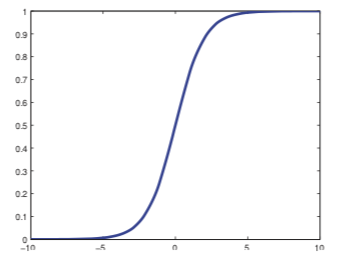
\includegraphics[width = 0.5\textwidth]{sigmoid.png}
  
  \caption {Gráfico da função sigmoid}

\end{figure}



\subsubsection{Função Custo}\hfill\newline
\hfill\newline

A função custo tem como objetivo quantificar a diferença entre o valor real e a predição. Esta função utiliza um vetor de pesos $\theta$, um vetor representativo da imagem $X$ e o valor da label associada a essa imagem $y$. Esta função começa por invocar um classificador logistico para obter uma predição $\hat{y}$. De seguida fazendo uso dos valores de $y$ e da probabilidade calculada da imagem pertencer a essa mesma classe $\hat{y}$ a diferença entre o valor real e o previsto é calculada da seguinte forma:
\hfill\newline
\hfill\newline
$E(\theta; e) = y*{\log_\epsilon (\hat{y})}+(1-y)*{\log_\epsilon (1-\hat{y})}$, em que $e$ é um evento composto por um par (X,y) respetivamente um vetor representativo de uma imagem e a label associada.

\hfill\newline
\hfill\newline
Como esta função é aplicada a toda a base de dados podemos generalizar a formula anterior para: 
\hfill\newline
\hfill\newline
$E(\theta; Base De Dados) = \frac{\sum_{n=0}^{N} y*{\log_\epsilon (\hat{y})}+(1-y)*{\log_\epsilon (1-\hat{y})}}{N}$

\hfill\newline
\hfill\newline

O vetor de pesos ($\theta$) ótimo é obtido através da minimização de uma função de custos que quantifica o erro entre a classe real e a sua predicção. O $\theta$ ideal é aquele que maximiza a probabilidade dos dados observados e denomina-se $\overline{\theta}$. \newline

\subsubsection{Atualização dos pesos}\hfill\newline
\hfill\newline

Para realizar a atualização dos pesos em classificadores logisticos é comum utilizar o método do gradiente, também chamado de método do declive que é utilizado para otimização. Para encontrar um mínimo local de uma função utiliza-se um esquema iterativo onde em cada passo se escolhe a direção negativa do gradiente a qual corresponde á direção de declive máximo. As seguintes definições explicam o processo de update dos pesos.\newline
\hfill\newline
Seja $\theta^0$ o vetor de pesos inicial e $\tau$ o learning rate usado pelo classificador logistico. Adcionalmente definimos $G$ como sendo a diferença entre o valor real $y$ e o valor da predição $\hat{y}$.\hfill\newline
\hfill\newline

$G = |y - \hat{y}|$ 
\hfill\newline
\hfill\newline

 A atualização dos pesos de $\theta^k$ para $\theta^{k+1}$ é feita então em duas etapas. A primeira atualiza a primeira componente $\theta_0$, e a segunda atualiza as restantes componentes de $\theta$\cite{ref2,ref4}.\hfill\newline
Relembrando as formulas anteriormente usadas para definir $\theta$ e o vetor de pixeis $X^m$ temos:\hfill\newline
\hfill\newline
$X^m=X_i^m, i=1,...,I$\hfill\newline
\hfill\newline
$\theta = (\theta_i),i=0,...,I$\hfill\newline
\hfill\newline
As formulas que mostram a atualização dos pesos definem-se como:\hfill\newline
\hfill\newline
$\theta_0(k+1) = \theta_0(k) + G \tau$\hfill\newline
\hfill\newline
$\theta_i(k+1) = \theta_i(k) + G \tau X_i,i=1,...,I$

\hfill\newline

Esta atualização de pesos é realizada $k$ vezes e quando $k$ tende para $\infty$, $\theta^k$ tende para $\overline{\theta}$ que corresponde ao array de pesos que minimizam o erro\cite{ref2}. Em notação simplificada:
 $k \xrightarrow{} \infty \Rightarrow \theta^k \xrightarrow{} \overline{\theta}$.\hfill\newline


%Os gráficos obtidos são do erro e função do k!! <-

\subsection{Matriz de Confusão}

A matriz de confusão é uma ferramenta muito utilizada em avaliações de modelos de previsão e é composta por quatro campos a saber\cite{ref9}:
\begin{itemize}
  \item Verdadeiro positivo (VP)\hfill\newline
  \hfill\newline
  Ocorre quando no conjunto real, a classe que pretendemos prever foi prevista corretamente.  \hfill\newline
  \item Verdadeiro negativo (VN)\hfill\newline
  \hfill\newline
  Ocorre quando no conjunto real, a classe que pretendemos prever foi prevista incorretamente.\hfill\newline
  \item Falso positivo (FP)\hfill\newline
  \hfill\newline
  Ocorre quando no conjunto real, a classe que não pretendemos prever foi prevista corretamente.\hfill\newline
  \item Falso negativo (FN)\hfill\newline
  \hfill\newline
  Ocorre quando no conjunto real, a classe que não pretendemos prever foi prevista incorretamente.\hfill\newline
\end{itemize}

A partir desta matriz podem-se calcular alguns valores importantes para avaliar a qualidade de predição do nosso modelo, esses valores são\cite{ref9}:

\begin{itemize}
  \item Accuracy\hfill\newline
  \hfill\newline
  Indica a taxa de sucesso das predições realizadas.\hfill\newline
  \hfill\newline
  $Accuracy = \frac{VP + FP}{VP+VN+FP+FN}$
  \hfill\newline
  \item Recall\hfill\newline
  \hfill\newline
  Indica a proporção de valores positivos corretamente identificados. Trata-se de uma boa métrica a aplicar em casos em que os Falsos Negativos são considerados mais prejudiciais que os Falsos Positivos.
  \hfill\newline
  \hfill\newline
  $Recall = \frac{VP}{VP+FN}$
  \hfill\newline
  \item Precisão\hfill\newline
  \hfill\newline
  Indica a percentagem de classificações positivas corretamente classificadas. Trata-se de uma boa métrica a aplicar em casos em que os Falsos Positivos são considerados mais prejudiciais do que os Falsos Negativos.
  \hfill\newline
  \hfill\newline
  $Precis\tilde{a}o = \frac{VP}{VP+FP}$
  \hfill\newpage
  \item F-score\hfill\newline
  \hfill\newline
  Esta métrica é uma média balanceada entre as métricas Recall e Precisão.
  \hfill\newline
  \hfill\newline
  $F\-score = 2*\frac{Precis\tilde{a}o * Recall}{Precis\tilde{a}o + Recall}$ 
\end{itemize}

Como exemplo de utilização desta matriz seja o array $Y$ o array de labels com os valores reais e seja $\hat{Y}$ o array de labels obtidas usando o classificador logistico, tendo ambos tamanho N. Convêm referir que caso o resultado de $\hat{y}(X^m,\theta) < 0.5$ a label $\hat{Y}_m$, correspondente á imagem $X^m$, será 0 e caso contrário será 1, uma vez que este indica a probabilidade de ser uma label e não a label em si\cite{ref2,ref3}. Assim a matriz de confusão será criada contabilizando em cada campo os valores que respeitarem as restrições apresentadas:


\begin{center}
 \resizebox{\textwidth}{!}{ %
 \begin{tabular}{||l|| c | c||} 
 \hline
 \backslashbox{Real}{Previsto} & Verdadeiro & Falso  \\ [0.5ex] 
 \hline\hline
 Verdadeiro & $Y_n == 1 \wedge \hat{Y}_n == 1, \forall n \in [0,N]$ & $Y_n == 1 \wedge \hat{Y}_n == 0, \forall n \in [0,N]$\\ 
 \hline
 Falso & $Y_n == 0 \wedge \hat{Y}_n == 1, \forall n \in [0,N]$ & $Y_n == 0 \wedge \hat{Y}_n == 0, \forall n \in [0,N]$ \\
 \hline
\end{tabular}%
  }
\end{center}




\section{Pooling}

Muitas vezes uma base de dados de imagens com imagens muito grandes (com um elevado número pixeis a serem processados) torna o processo de previsão, análise de custos e update de pesos bastante demorado\cite{ref8}.\newline
A técnica de pooling permite dividir uma imagem em várias mais pequenas através de uma janela deslizante e aplicar um filtro a cada uma de forma a remover o ruido, manter a informação útil e reduzir a dimensão da imagem a analisar\cite{ref8}.\newline
Seja $B$ uma imagem composta por pixeis a ser processada por pooling e $A$ uma janela deslizante, com dimensões inferiores a $B$, a ser usada no processo, isto é o número de pixeis da janela $A$ é inferior ao número de pixeis de $B$.\newline
O deslize da janela $A$ sobre a imagem original é determinado por um stride horizontal e um stride vertical. A cada sub-imagem obtida pela aplicação de $A$ a $B$ é posteriormente aplicado um filtro que permite obter um valor a partir dos pixeis existentes na sub-imagem, este processo denomina-se pooling. No final, juntando todos os resultados obtidos pelo filtro, obtemos uma imagem reduzida $C$ que será utilizada para realizar a classificação pretendida.\newline
Em baixo podemos visualizar, na imagem a), um exemplo da aplicação de um filtro a uma janela\cite{ref8}, já na segunda imagem apresentada é representado um exemplo da aplicação de um filtro á janela deslizante de tamanho 3x3 com um stride de 2 ao longo de uma das dimensões da imagem\cite{ref8}.

\begin{figure}[H]

  
  \captionsetup{justification=centering}
  \captionsetup{justification=centering}
  \begin{subfigure}{.5\textwidth}
  \centering
  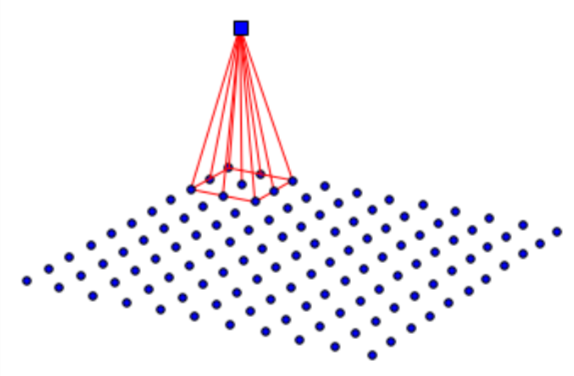
\includegraphics[width = 0.8\textwidth]{aplicacaoFiltro.png}
  \caption {Exemplo de aplicação de um filtro a uma janela sobre uma imagem representada por pixeis}
  \end{subfigure}
  \begin{subfigure}{.5\textwidth}
  \centering
   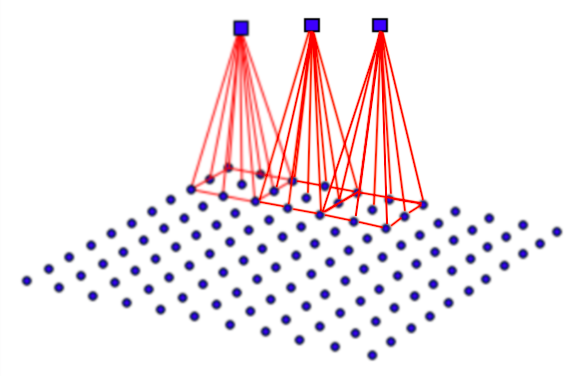
\includegraphics[width = 0.8\linewidth, height=3.3cm]{aplicacaostride.png}
   \caption {Exemplo de aplicação de pooling a uma imagem representada por pixeis}
   \end{subfigure}

\end{figure}

Num exemplo mais concreto, em baixo, podemos ver uma imagem cujas dimensões são 30 x 30, essa imagem foi tratada com uma janela deslizante de 3 x 3 e um stride de 3 nos eixos x e y resultando em 100 imagens a serem processadas pelo filtro escolhido.\newline
Como já foi referido cada filtro recebe uma sub-imagem correspondente aos pixeis abrangidos pela janela deslizante e devolve um valor, cada valor devolvido será posteriormente recolhido pela ordem em que cada sub-imagem foi filtrada de forma a refazer a figura com as caracteristicas obtidas através dos filtros. Em baixo podemos observar um esquema resumido de todo o processo de pooling.  

\begin{figure}[H]

  \centering
  \captionsetup{justification=centering}

  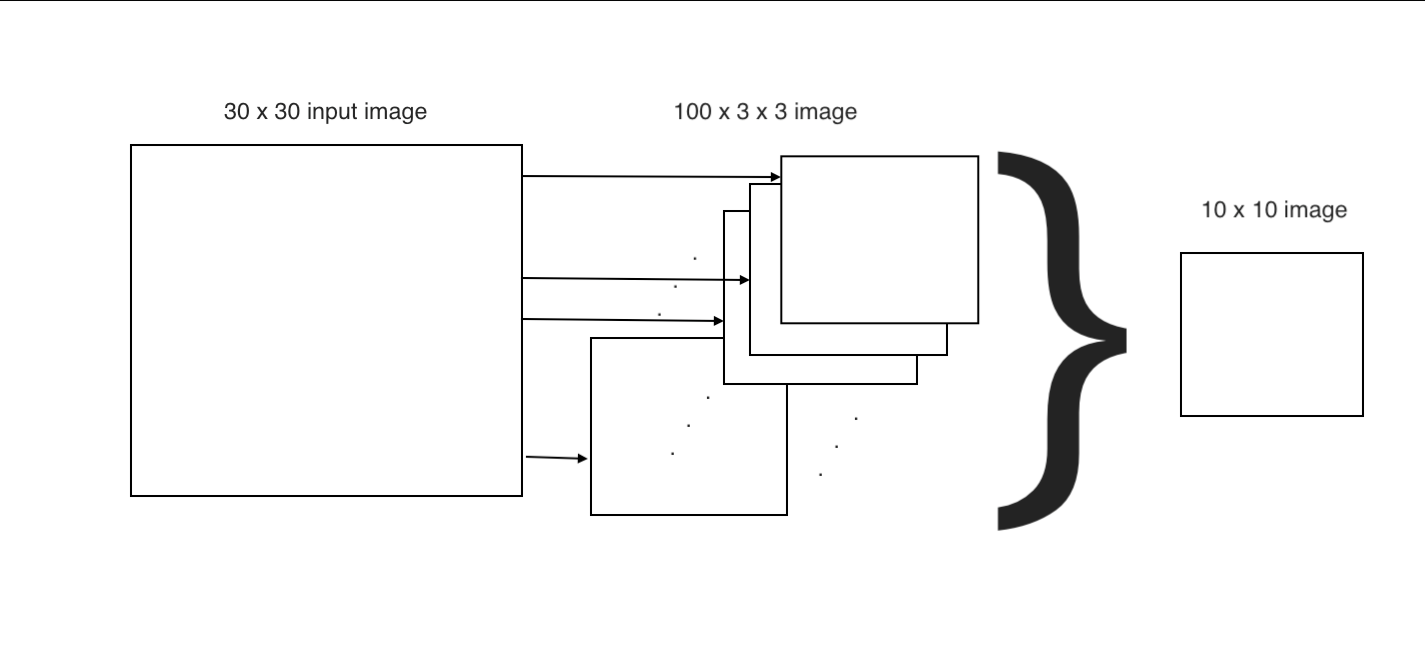
\includegraphics[width = 0.8\textwidth]{pooling.png}
  
  \caption {Esquema básico de pooling}

\end{figure}

\subsection{Poolings Clássicos}\hfill\newline
\hfill\newline
\label{subsec:poolingClassico}

Existem alguns pooling classicos que são comummente usados como o "max-pooling", "min-pooling", "average-pooling" e "maximum centered pooling", todos eles serão em seguida explicados.

\subsubsection{Max-Pooling}\hfill\newline
  \hfill\newline
  O max pooling trata-se de um filtro aplicado a uma imagem que devolve o valor máximo dessa imagem, isto é, como cada imagem consiste num conjunto de pixeis cujos valores variam dentro do intervalo de números inteiros [0,255] o max-pooling vai devolver o valor mais alto contido na imagem\cite{ref8}. Seja $A$ uma janela de pixeis que representa uma parte de uma imagem, a formula deste filtro aplicado a $A$ é a seguinte:\hfill\newline
  \hfill\newline
  $max\_pooling(A) = max(A)$
  \hfill\newline
  \hfill\newline
  Um exemplo deste tipo de filtro pode ser visualizado em baixo.

  \begin{figure}[H]

    \centering
    \captionsetup{justification=centering}

    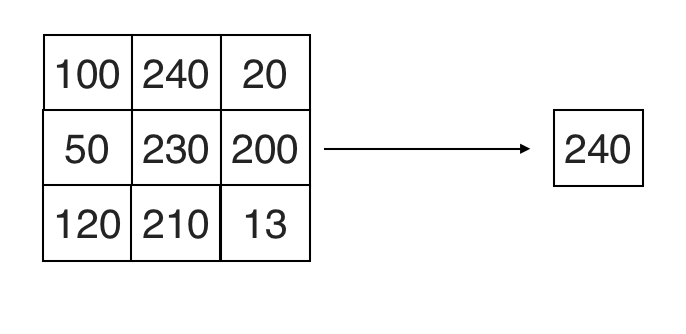
\includegraphics[width = 0.8\textwidth]{maxpooling.png}
    
    \caption {Exemplo de Max-Pooling}

  \end{figure}


\subsubsection{Min-Pooling}\hfill\newline
  \hfill\newline
  O min-pooling trata-se de um filtro aplicado a uma imagem que devolve o valor minimo contido nessa mesma imagem, isto é, dos valores dos pixeis da imagem é devolvido o menor. Seja $A$ uma janela de pixeis  que representa uma parte de uma imagem, a formula deste filtro aplicado a $A$ é a seguinte:\hfill\newline
  \hfill\newline
  $min\_pooling(L) = min(A)$
  \hfill\newline
  \hfill\newline
  Em baixo pode-se observar um exemplo deste filtro.

  \begin{figure}[H]

    \centering
    \captionsetup{justification=centering}

    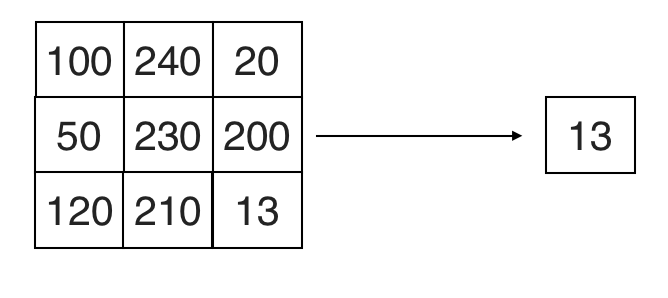
\includegraphics[width = 0.8\textwidth]{minpooling.png}
    
    \caption {Exemplo de Min-Pooling}

  \end{figure}


\subsubsection{Average Pooling}\hfill\newline
  \hfill\newline
  O average pooling trata-se de um filtro aplicado a uma imagem que devolve o valor médio dos pixeis dessa imagem, isto é, os valores de todos os pixeis são somados e posteriormente são divididos pelo número de pixeis existentes na imagem para obter uma média por pixel\cite{ref8}. Seja $A$ uma janela de pixeis de uma parte de uma imagem com dimensões $L1$ e $L2$, a formula deste filtro aplicado a $A$ é a seguinte:\hfill\newline
  \hfill\newline
  $average\_pooling(A) = \frac{\sum_{i=0}^{L1}\sum_{j=0}^{L2} A_{ij}}{L1*L2}$
  \hfill\newline
  \hfill\newline
  Um exemplo deste filtro pode ser visualizado em baixo.

  \begin{figure}[H]

    \centering
    \captionsetup{justification=centering}

    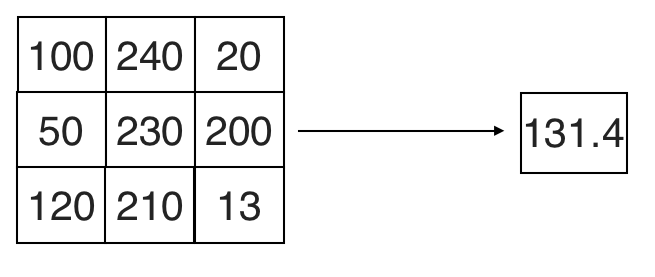
\includegraphics[width = 0.8\textwidth]{avgpooling.png}
    
    \caption {Exemplo de Average Pooling}

  \end{figure}


\subsubsection{Maximum Centered Pooling}\hfill\newline
  \hfill\newline
  O maximum minus average pooling trata-se de um filtro aplicado a uma imagem que devolve o valor médio dessa imagem subtraido ao valor máximo da mesma, isto é, primeiro acha-se a média dos pixeis da imagem e o valor máximo de todos esses pixeis e devolve-se a diferença entre o valor máximo encontrado e a média dos valores de todos os pixeis da imagem.Seja $A$ uma janela de pixeis de uma parte de uma imagem com dimensões $L1$ e $L2$, a formula deste filtro aplicado a $A$ é a seguinte:\hfill\newline
  \hfill\newline
  $max\_centered\_pooling(A) = max(A) - \frac{\sum_{i=0}^{L1}\sum_{j=0}^{L2} A_{ij}}{L1*L2}$
  \hfill\newline
  \hfill\newline
  Em baixo é apresentado um exemplo simples da aplicação deste filtro.

  \begin{figure}[H]

    \centering
    \captionsetup{justification=centering}

    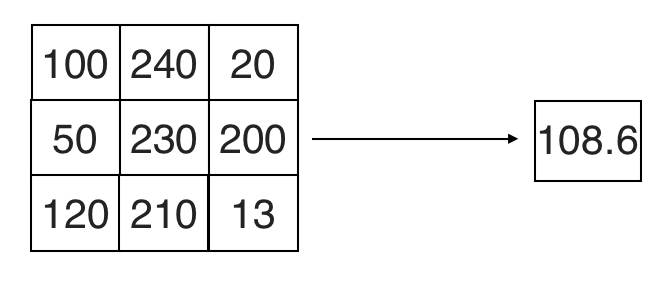
\includegraphics[width = 0.8\textwidth]{maxavgpooling.png}
    
    \caption {Exemplo de Maximum Centered Pooling}
  \end{figure}


\subsection{Poolings Exóticos}
\label{subsec:poolingExotico}

Existem também alguns poolings exóticos definidos especificamente para a base de dados que possuimos. Estes não funcionam da mesma maneira que os classicos uma vez que se baseiam em caracteristicas das imagens do dataset. \newline
Como o dataset é constituido de imagens do número 3 e do número 8 e a diferença na representação dos mesmos, de forma simplista, pode ser entendida com se tratando de que no oito temos dois circulos fechados e no três temos dois circulos com cerca de um quarto dos mesmos por concluir, sendo a junção dos circulos sobreposta de igual forma com se pode ver nas figuras abaixo.

\begin{figure}[H]

  %\centering
  \captionsetup{justification=centering}
  \begin{subfigure}{.5\textwidth}
  \centering
  
\includegraphics[width = 0.4\linewidth, height=3cm]{3.png}
  \end{subfigure}
  \begin{subfigure}{.5\textwidth}
  \centering
   
\includegraphics[width = 0.4\linewidth, height=3.3cm]{8.png}
   \end{subfigure}
  \caption {Representação dos números 3 e 8}
\end{figure}

Isto fornece-nos algumas ideias sobre os tipos de filtros que se podem criar tendo em conta esta simplificação das diferenças dos mesmos.


\subsubsection{ Diagonal and Vertical Average Pooling}\hfill\newline
  \hfill\newline
  Neste primeiro filtro a ideia subjacente passa por, tentar utilizar a diferença dos valores dos pixeis do oito e do 3 verticalmente e diagonalmente tal como se pode ver nas figuras abaixo que identificam o que esperamos encontrar. \hfill\newline

  \begin{figure}[H]

      %\centering
      \captionsetup{justification=centering}
      \begin{subfigure}{.5\textwidth}
        \centering
        
\includegraphics[width = 0.4\linewidth, height=3cm]{3_1.png}
        \end{subfigure}
        \begin{subfigure}{.5\textwidth}
        \centering
         
\includegraphics[width = 0.4\linewidth, height=3.3cm]{8_1.png}
      \end{subfigure}
      \begin{subfigure}{.5\textwidth}
        \centering
        
\includegraphics[width = 0.5\linewidth, height=3.5cm]{3_2.png}
        \end{subfigure}
        \begin{subfigure}{.5\textwidth}
        \centering
         
\includegraphics[width = 0.5\linewidth, height=3.8cm]{8_2.png}
      \end{subfigure}
      \caption {Representação do objetivo a identificar como o filtro sobre os números 3 e 8}
  \end{figure}

  A pensar neste tipo de abordagem este filtro soma os eixos diagonal (sentido descendente da esquerda para a direita) e vertical da janela recebida e divide os mesmos pelo número de elementos somados. Seja $A$ a janela de dimensões $size\_x$ e $size\_y$. As seguintes formulas mostram os passos para a realização do processo.\newline
  Posição inicial da lista vertical:\hfill\newline
  \hfill\newline
  $p\_vertical = size\_x : 2$, em que o valor p\_vertical é arredondado ás unidades.\hfill\newline
  \hfill\newline
  Posição inicial da lista diagonal:\hfill\newline
  \hfill\newline
  $p\_diagonal = 0$\hfill\newline
  \hfill\newline
  Deve existir um elemento que dite a linha da matriz a consultar começando inicializado a 0:\hfill\newline
  \hfill\newline
  $linha = 0$\hfill\newline
  \hfill\newline
  Deve ainda existir 1 lista para armazenar os pixeis verticais e diagonais, cujo comprimento é $L = 0$.\hfill\newline
  \hfill\newline
  $lista = []$\hfill\newline
  \hfill\newline
  A cada iteração a lista com os pixeis diagonais e verticais, que no inicio do processo se encontra vazia é atualizada acrescentando dois elementos da matriz $A$, fazendo com que o seu comprimento $L$ aumente também em 2 unidades.Adicionalmente a variável linha também aumenta em 1 unidade.\hfill\newline
  \hfill\newline
  $lista(k+1) = lista(k) + [ A_{p\_diagonal,linha}] + [ A_{p\_vertical,linha}]$\hfill\newline
  $L(k+1) = L(k) + 2$\hfill\newline
  $linha(k+1) = linha(k) + 1$\hfill\newline
  \hfill\newline
  No final é realizada a soma dos elementos da lista e a divisão  desta soma pelo número de elementos da mesma.\hfill\newline
  \hfill\newline
  $media = \frac{\sum_{i=0}^{L} lista_i}{L}$\hfill\newline
  \hfill\newline

  A variável media é devolvido pelo filtro como o resultado do processamento da janela.


\subsubsection{Diagonal and Vertical Max Centered Pooling}\hfill\newline
  \hfill\newline
  Á semelhança do filtro anterior este filtro também pretende usar a diagonal e a vertical do vetor representativo da janela deslizante, a diferença é que este subtrai a média, que é calculada da mesma forma que na função anterior, ao valor máximo encontrado na diagonal e vertical da janela representada pelo vetor. Assim, reaproveitando todas as definições anteriormente apresentadas o resultado devolvido por este filtro é:\hfill\newline
  \hfill\newline
  $max\_centered = max(lista) - media$



\subsubsection{Diagonal and Vertical Max Pooling}\hfill\newline
  \hfill\newline
  Este filtro parte do principio que as imagens representativas dos números 3 e 8 podem ser dadas rotacionadas em qualquer direção e para tentar mitigar esse problema são calculas ambas as diagonais e a vertical colecionando-as em arrays distintos, verifica qual o valor mínimo de cada um dos arrays colecionados e posteriormente devolve o maximo valor dos 3 anteriormente obtidos. As definições das seguintes formulas são dadas pela ordem de implementação:\hfill\newline 
  \hfill\newline
  Posição inicial da lista vertical $V1 $:\hfill\newline
  \hfill\newline
  $p\_vertical = size\_x : 2$, em que o valor p\_vertical é arredondado ás unidades.\hfill\newline
  \hfill\newline
  Valor a ser usado para calcular as posições dos pixeis de ambas as listas diagonais $D1$ e $D2$:\hfill\newline
  \hfill\newline
  $p\_diagonal = 0$\hfill\newline
  \hfill\newline
  Deve existir um elemento que dite a linha da matriz a consultar começando inicializado a 0:\hfill\newline
  \hfill\newline
  $linha = 0$\hfill\newline
  \hfill\newline
  Devem ainda existir 3 listas para armazenar os pixeis verticais e diagonais, cujos comprimentos são 0 aquando da sua criação.\hfill\newline
  \hfill\newline
  $V1 = []$\hfill\newline
  $D1 = []$\hfill\newline
  $D2 = []$\hfill\newline
  \hfill\newline
  A cada iteração as listas são incrementadas em 1 elemento. Adicionalmente a variável linha também aumenta em 1 unidade.\hfill\newline
  \hfill\newline
  $V1(k+1) = V1(k) + [ A_{p\_vertical,linha}]$\hfill\newline
  $D1(k+1) = D1(k) + [ A_{p\_diagonal,linha}]$\hfill\newline
  $D2(k+1) = D2(k) + [ A_{size\_x-(p\_diagonal+1),linha}]$\footnote{Note-se que é necessário somar uma unidade a $p\_diagonal$ uma vez que o primeiro elemento de A se encontra na posição 0 fazendo com que o último elemento de uma linha da matriz se encontre numa posição múltipla de $size\_x-1$ e não de $size\_x$}\hfill\newline
  $linha(k+1) = linha(k) + 1$\hfill\newline
  \hfill\newline
  No final é devolvido o pixel com valor máximo das 3 listas criadas.\hfill\newline
  \hfill\newline
  $maximum = max(max(max(V1),max(D1)),max(D2))$\hfill\newline
  \hfill\newline
\newpage

\subsubsection{Diagonal and Vertical Min Average Pooling}\hfill\newline
  \hfill\newline
  Á semelhança do filtro anterior, este filtro calcula 3 arrays correspondentes ás diagonais e á vertical. Em seguida realiza a média de cada um dos arrays e devolve a menor média. Assim, reaproveitando as definições anteriormente feitas sobre os arrays $V1$, $D1$ e $D2$ e sobre as respetivas atualizações a cada iteração temos as seguintes definições:\hfill\newline
  Para cada lista é necessário calcular a média. Note-se que cada lista possui o mesmo comprimento pois foi recolhido 1 pixel por linha para cada uma. Seja $Dim1$ a dimensão da lista $V1$ assim:\hfill\newline
  \hfill\newline
  $M1 = \frac{\sum_{i=0}^{Dim1} V1_i}{Dim1}$ \hfill\newline
  $M2 = \frac{\sum_{i=0}^{Dim1} D1_i}{Dim1}$ \hfill\newline
  $M3 = \frac{\sum_{i=0}^{Dim1} D2_i}{Dim1}$ \hfill\newline
  \hfill\newline
  Por fim é realizada a escolha da menor média obtida. \hfill\newline
  \hfill\newline
  $menor\_media = min(min(M1,M2),M3)$ \hfill\newline
  \hfill\newline

\newpage
\input{Objetivo.tex}
\newpage
\section{Implementação}

Nesta secção mostrar-se-á a implementação em python da preparação da base de dados, do classificador logistico, das funções de pooling e das funções de avaliação da performance dos modelos.

\subsection{Base de Dados}

A base de dados utilizada neste trabalho possui 2000 imagens das quais 1000 representam o número 3 e as restantes 1000 repreentam o número 8. A cada imagem que representa o número 3 foi atribuida a label 0 e ás restantes atribuiu-se a label 1 fazendo desta uma base de dados binária.\newline
Cada imagem do dataset é composta por 36 colunas e 31 linhas totalizando 1116 pixeis cujos valores variam entre 0 e 255.


\subsection{Prepare data}

Foi criada uma função que permitisse separar as imagens e respetivas labels em datasets de treino e teste, um procedimento necessário para criar um dataset de validação que nos permita escolher o melhor modelo\cite{ref2,ref6}. Esta função recebe um vetor com as imagens\footnote{Note-se que as imagens já estão baralhadas no dataset antes de serem passadas á função em questão.}, um vetor com as labels correpondentes ás imagens, o número de imagens no vetor, as dimensões das imagens e a percentagem das imagens a serem usadas para treino.\newline
Esta função calcula o número de imagens a serem utilizadas para treino com base na percentagem recebida, separando assim as imagens e respetivas labels em dataset de treino e teste. Neste caso foram utilizadas 85\% das imagens para treino e os restantes 15\% foram utilizados para teste\cite{ref6}. \newline
É criado um array de pesos $ew$ com o mesmo número de elementos que uma imagem a partir das dimensões recebidas pela função e é avaliado um erro para o array de pesos iniciais.\newline
Esta função devolve os datasets de treino e teste bem como os respetivos tamanhos o array de pesos e o erro inicial.
\begin{figure}[H]

  \centering
  \captionsetup{justification=centering}

  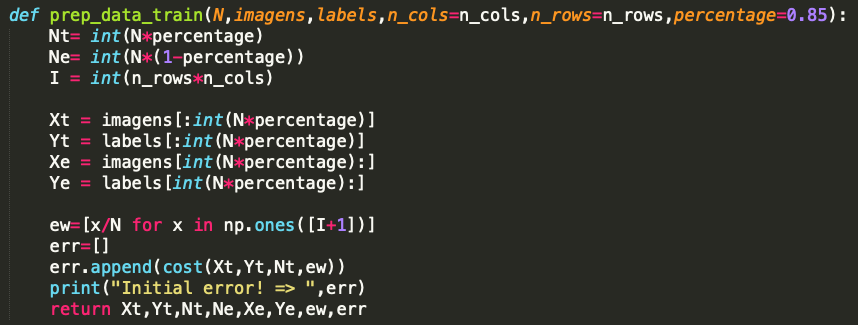
\includegraphics[width = \textwidth]{f_prep_data.png}
  
  \caption {Função de preparação dos datasets de treino e teste}
\end{figure}

\subsection{Classificador Logistico}


A implementação do classificador logistico foi dividida em 5 funções, nomeadamente: $run\_stocastic$, $predictor$, $sigmoid$, $cost$ e $update$ . Estas funções e respetivos funcionamentos serão apresentados em seguida pela ordem em que foram referidos.\newline



\subsubsection{Run Stocastic}\hfill\newline
	\hfill\newline

	A função run\_stocastic trata-se da função principal da implementação do classificador logistico e tal como o nome indica aplica o método estocástico ao mesmo. O método estocástico foi escolhido porque se trata do método que apresenta o menor custo em termos de performance face ás restantes tecnologias\cite{ref6,ref7}.\newline
	Esta função começa por definir que o erro almejado tem valor 0, indicando assim uma das condições de paragem do ciclo. Começa também por criar um contador $it$ para contabilizar as iterações realizadas inicializando este a 0.\newline
	A cada iteração é escolhido um elemento aleatório da nossa base de dados de treino e é calculado um novo vetor de pesos recorrendo á função $update$. Este novo vetor é posteriormente utilizado para calcular um erro através da função custo que indica a diferença entre os valores das labels calculados com recurso aos novos pesos e os valores reais das labels, sendo este erro armazenado para posterior visualização. A variável $it$ é então incrementada em 1 unidade e caso tenha atingido o número máximo de iterações que pretendemos sai do ciclo. 
	No final é devolvido o array de pesos juntamente com o array que contêm a progressão dos erros ao longo das iterações realizadas.

	\begin{figure}[H]

	  \centering
	  \captionsetup{justification=centering}

	  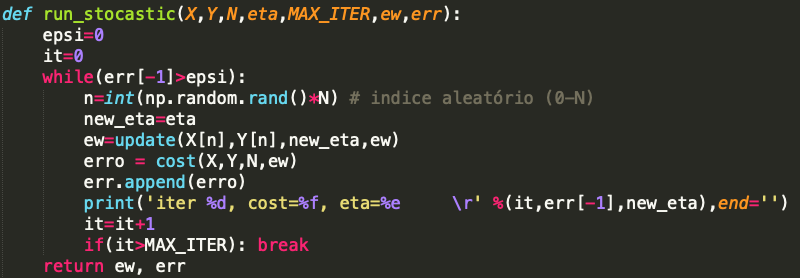
\includegraphics[width = \textwidth]{f_stocastic.png}
	  
	  \caption {Função Estocástica implementada}
	\end{figure}



\subsubsection{Predictor}\hfill\newline
	\hfill\newline

	A função predictor é responsável por calcular o valor em $\mathbb{R}$ a ser passado á função sigma. Este valor em $\mathbb{R}$ é calculado fazendo a soma do primeiro elemento do vetor de pesos pelo produto vetorial dos restantes elementos desse vetor com o array de pixeis representativo da imagem. No fim é devolvido o resultado de sigma.

	\begin{figure}[H]

	  \centering
	  \captionsetup{justification=centering}

	  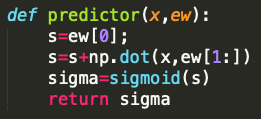
\includegraphics[width = 0.4\textwidth]{f_predictor.png}
	  
	  \caption {Função Predictor implementada}
	\end{figure}


\subsubsection{Sigmoid}\hfill\newline
	\hfill\newline
	Para a sua implementação recorreu-se á biblioteca python $numpy$ que possui uma função $numpy.exp()$ que recebe um expoente $s$ e calcula $e^s$, no entanto foi necessário ter atenção á capacidade de precisão do computador\footnote{A capacidade de precisão do computador refere-se ao número máximo de bits disponíveis para a representação de um número, exceder esta capacidade leva a erros de \textit{Overflow}.} e por esse motivo criaram-se limites de expoente de forma a que este não excedesse os números 30 e -30. \newline
	Nesta função o valor de s é arredondado mediante a necessidade, como referido no parágrafo anterior, e é usado como expoente de $\epsilon$ na função $\sigma$ devolvendo o resultado da mesma.

	\begin{figure}[H]

	  \centering
	  \captionsetup{justification=centering}

	  \includegraphics[width = 0.5\textwidth]{f_sigmoid.png}
	  
	  \caption {Função Sigmoid implementada}
	\end{figure}


\subsubsection{Cost}\hfill\newline
	\hfill\newline
	Esta função começa por criar um acumulador para os erros de predição das labels das imagens face ás labels reais chamado $En$ que é inicializado a 0 e pelos mesmos motivos de precisão computacional da função sigmoid establece um limite mínimo e máximo para o valor previsto.\newline
	Em seguida é iterado todo o dataset de treino imagem a imagem e sobre cada uma é calculada a probabilidade de esta imagem pertencer á label 1 e é utilizada a formula $Y_n*\log_\epsilon(\hat(y))+(1-Y_n)*\log_\epsilon{1-\hat(y)}$ para calcular o desvio da predição somando-o á variável $En$.\newline
	No fim é devolvida a média dos erros dividindo os erros acumulados pelos número de imagem iteradas.

	\begin{figure}[H]

	  \centering
	  \captionsetup{justification=centering}

	  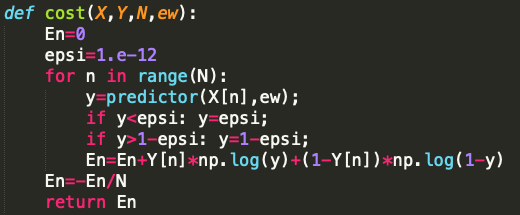
\includegraphics[width = 0.7\textwidth]{f_cost.png}
	  
	  \caption {Função Cost implementada}
	\end{figure}


\subsubsection{Update}\hfill\newline
	\hfill\newline
	A função update começa por obter uma predição sobre uma imagem e calcula a diferença entre o valor real da label da imagem e o valor previsto guardando-o na variável $s$. A variável $eta$ representa o learning rate a ser usado na atualização dos pesos.\newline
	 Posteriormente o primeiro elemento do array de pesos é atualizando somando-se ao produto de $s$ por $eta$ e os restantes elementos do array de pesos são atualizados individualmente somando-se ao produto de $s$ com $eta$ com o elemento da imagem x que se encontra na mesma posição do array - 1.\newline
	No final é devolvido um array com os pesos atualizados.

	\begin{figure}[H]

	  \centering
	  \captionsetup{justification=centering}

	  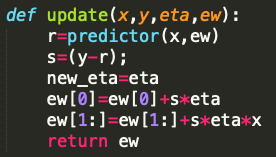
\includegraphics[width = 0.4\textwidth]{f_update.png}
	  
	  \caption {Função Update implementada}
	\end{figure}



\subsection{Poolings Clássicos}

 Nesta subsecção explicar-se-á a implementação das técnicas de pooling clássicas referidas na secção anterior. É de notar que a matriz a que cada pooling é aplicado foi transformada numa lista para uma mais facil implementação.


\subsubsection{Max Pooling}\hfill\newline
	\hfill\newline
	Este filtro aplica a função $max$ do python á lista recebida.

	\begin{figure}[H]

	  \centering
	  \captionsetup{justification=centering}

	  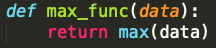
\includegraphics[width = 0.3\textwidth]{f_max.png}
	  
	  \caption {Função Max implementada}
	\end{figure}

\subsubsection{Min Pooling}\hfill\newline
	\hfill\newline

	Este filtro aplica a função $min$ do python á lista recebida.

	\begin{figure}[H]

	  \centering
	  \captionsetup{justification=centering}

	  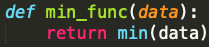
\includegraphics[width = 0.3\textwidth]{f_min.png}
	  
	  \caption {Função Min implementada}
	\end{figure}

\subsubsection{Average Pooling}\hfill\newline
	\hfill\newline

	Este filtor realiza uma divisão entre a soma dos elementos do vetor recebido e o tamanho do vetor recebido.


	\begin{figure}[H]

	  \centering
	  \captionsetup{justification=centering}

	  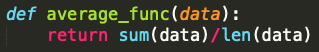
\includegraphics[width = 0.5\textwidth]{f_avg.png}
	  
	  \caption {Função Average implementada}
	\end{figure}

\subsubsection{Max Centered Pooling}\hfill\newline
	\hfill\newline

	Neste filtro utilizaram-se dois filtros préviamente definidos, subtraindo o resultado do filtro de average pooling ao resultado do filtro de max pooling. 


	\begin{figure}[H]

	  \centering
	  \captionsetup{justification=centering}

	  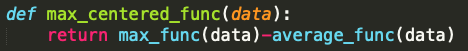
\includegraphics[width = 0.7\textwidth]{f_max_centered.png}
	  
	  \caption {Função Max centered implementada}
	\end{figure}



\subsection{Poolings Exóticos}\hfill\newline
\hfill\newline

Tal como já se referiu anteriormente foram criados alguns filtros de pooling exóticos baseados nas características do dataset de imagens. A sua implementação é decrita a seguir.

\subsubsection{ Diagonal and Vertical Average Pooling}\hfill\newline
  \hfill\newline

  A implemetação deste filtro passou por criar uma lista vazia denominada $lista$, uma variável $pos$\footnote{note-se que foi tirado partido do facto de a posição da diagonal ter as mesmas coordenadas em x e y, logo a variavel $pos$ representa tanto a linha da matriz em que estamos como a posição na linha em que o pixel se encontra.} a utilizar para iterar a posição do pixel a adicionar pertencente á diagonal da janela e uma variável $center$ que indica a posição do pixel de cada linha pertencente á vertical que se encontra no centro da janela.\newline
  Posteriormente é realizado um ciclo enquanto a posição do pixel diagonal for inferior a ambas as dimensões da janela. Em cada iteração, começa-se por adicionar á lista o pixel diagonal calculado como a posição do pixel diagonal na linha $pos$ somado com o número de pixeis por linha já percorrida. Em seguida acrescenta-se á lista o pixel pertencente á vertical calculado como a posição na linha correspondente á vertical dada pela variável $center$ somada ao número de pixeis percorridos nas linhas anteriores. Note-se que existe sempre um ponto em que a diagonal e a vertical se intersetam, o problema da dupla contabilização deste ponto foi resolvido com um if que impede que tal aconteça.\newline

   No final de cada iteração a linha, representada pela variável $pos$, é atualizada sendo incrementada em 1 unidade.\newline
  No fim da função retorna-se a média dos elementos da lista.

	\begin{figure}[H]

	  \centering
	  \captionsetup{justification=centering}

	  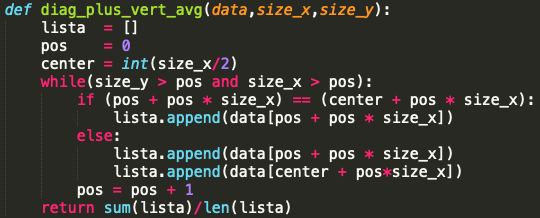
\includegraphics[width = 0.7\textwidth]{f_diag_plus_vert.png}
	  
	  \caption {Função que realiza a média sobre o filtro diagonal e vertical}
	\end{figure}


\subsubsection{Diagonal and vertical Max Centered Pooling}\hfill\newline
  \hfill\newline
  Esta função começa, tal como a anterior, por definir uma lista vazia, uma variável $pos$ e uma variável $center$ seguindo-se a coleta dos elementos da diagonal superior e da vertical da janela durante o ciclo que se segue. No final é devolvida a diferença entre o valor máximo da lista e a média dos valores da mesma.


    \begin{figure}[H]

	  \centering
	  \captionsetup{justification=centering}

	  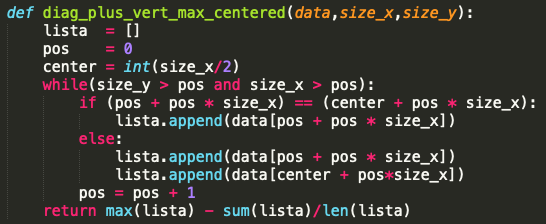
\includegraphics[width = 0.7\textwidth]{f_diag_plus_vert_max_centered.png}
	  
	  \caption {Função que realiza o "Max centered" sobre filtro diagonal e vertical}
    \end{figure}


\subsubsection{Diagonal and Vertical Max Pooling}\hfill\newline
  \hfill\newline
  	Nesta função são declaradas 3 listas, sendo que cada uma vai conter os elementos de uma das diagonais ou os elementos da reta vertical que se encontra no centro da janela. É também declarada uma variável $pos$ e uma variável $center$ á semelhança dos restantes filtros exóticos.\newline
  	Durante o ciclo os elementos da diagonal decrescente são colecionados no array $diag1$, os elementos da diagonal crescente no array $diag2$ sendo os elementos da vertical armazenados no array $vert$. \newline
  	Após o ciclo é encontrado o valor mínimo de cada um dos 3 arrays e desses é devolvido o maior.


	\begin{figure}[H]

	  \centering
	  \captionsetup{justification=centering}

	  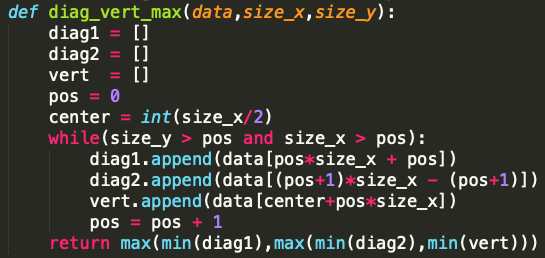
\includegraphics[width = 0.8\textwidth]{f_diag_vert_max.png}
	  
	  \caption {Função que obtem o maximo valor dos 3 valores mínimos encontrados nas diagonais e vertical do vetor}
	\end{figure}


\subsubsection{Diagonal and Vertical Min Average Pooling}\hfill\newline
  \hfill\newline
  Nesta função á semelhança da anterior declararam-se 3 listas, uma variavel $pos$ e uma variável $center$ que desempenham o mesmo papel que na função anterior. A coleta e armazenamento dos elementos das diagonais e da coluna central da janela também foram realizadas da mesma forma que na função anterior.\newline
  Após o ciclo foi calculada a média de cada lista e foi devolvida a menor média das três.

	\begin{figure}[H]

	  \centering
	  \captionsetup{justification=centering}

	  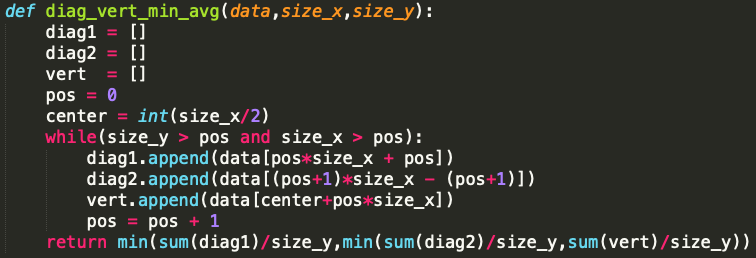
\includegraphics[width = \textwidth]{f_diag_vert_min_avg.png}
	  
	  \caption {Função que obtem o minimo valor das 3 médias calculadas sobre as diagonais e vertical do vetor}
	\end{figure}


Foi ainda definida uma função que permite simplificar a escolha do filtro a ser usado, ou seja, dada uma opção numérica, aplica o filtro associado ao vetor representativo da janela deslizante.

\begin{figure}[H]

  \centering
  \captionsetup{justification=centering}

  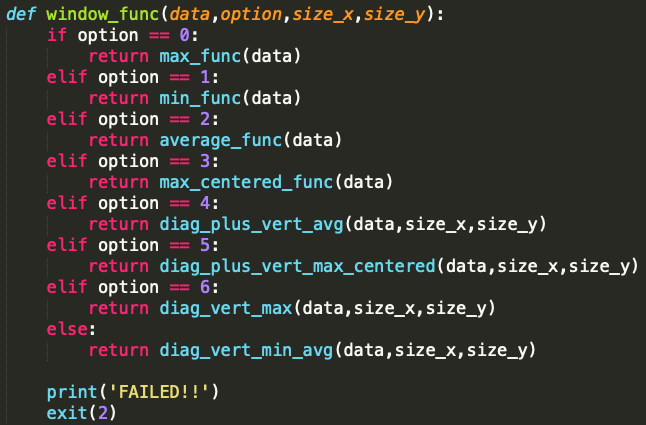
\includegraphics[width = 0.8\textwidth]{f_windows.png}
  
  \caption {Função responsável por fazer a correspondência opção-filtro}
\end{figure}


\subsubsection{Janela Deslizante}\hfill\newline
    \hfill\newline

	Foi implementada uma função responsável por aplicar a janela deslizante a cada imagem do dataset de forma genérica.\newline
	Esta função começa por definir as dimensões da imagem pós-filtro calculando quantas vezes tem de somar o $stride\_x$ á dimensão $x$ da janela deslizante para atingir o mesmo número de colunas que a imagem original e o mesmo processo é aplicado para calcular as dimensões em $y$ da imagem pós-filtro, fazendo uso da dimensão $y$ da janela, da variavel $stride\_y$ e da dimesão em $y$ da imagem pré-filtro\cite{ref8}.\newline
	Posteriormente os vetores representativos das imagens originais são iterados um a um e para cada são calculadas as posições abrangidas pela janela a cada iteração começando no ponto inicial (0,0) até a janela ter percorrido a totalidade da imagem. A cada uma das referidas iterações, nas quais se movimenta a janela, os pixeis abrangidos pela janela são armazenados num vetor ao qual se aplica um filtro para obter o valor de um pixel que passará a integrar a imagem pós-filtro.\newline
	O novo dataset constituido pelas imagens pós-filtro é então devolvido pela função.


	\begin{figure}[H]

	  \centering
	  \captionsetup{justification=centering}

	  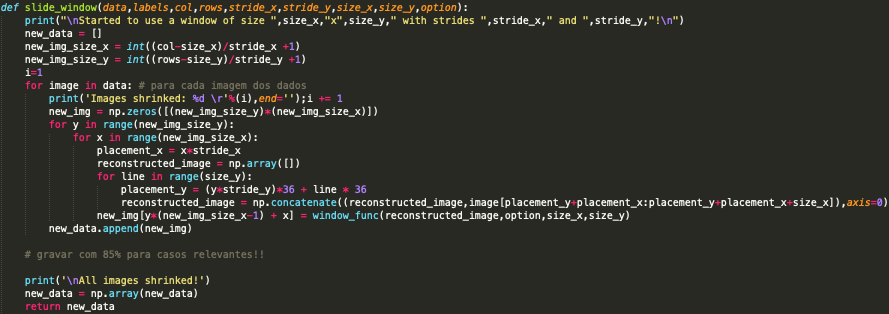
\includegraphics[width = \textwidth]{f_slidewindow.png}
	  
	  \caption {Função responsável por executar a janela deslizante}
	\end{figure}


\subsection{Avaliação de Resultados}

Para avaliar os modelos criados foi implementada uma função que calcula a matriz de confusão. Uma vez que no dataset utilizado classificar mal um 3 e classificar mal um 8 tem o mesmo peso a métrica Accuracy é a ideal para avaliar a qualidade das previsões do modelo, as métrica de Recall, Precisão e F-Score não são as melhores a aplicar uma vez que atribuem inportancias diferentes á classificação errónea de um 3 ou um 8.

\subsubsection{Matriz de Confusão}\hfill\newline
\hfill\newline

Esta função começa por criar a matriz 2x2 onde serão contabilizados os resultados da previsão das diversas imagens consoante se enquadrem nas definições dadas para o preenchimento de cada campo da matriz. Note-se que cada camp é inicializada a 0.\newline
As imagens da dataset são iteradas uma a uma e para cada é realizada um previsão. Posteriormente é contabilizado na tabela de confusão um dos quatro resultados:
\begin{itemize}
  \item Caso a previsão seja inferior a 0.5 e a label também a posição (0,0) da matriz é incrementada em um unidade.
  \item Caso a previsão seja superior a 0.5 e a label também a posição (1,1) da matriz é incrementada em um unidade.
  \item Caso a previsão seja inferior a 0.5 e a label seja superior a 0.5 a posição (0,1) da matriz é incrementada em um unidade.
  \item Caso a previsão seja superior a 0.5 e a label não a posição (1,0) da matriz é incrementada em um unidade.
\end{itemize}

\begin{figure}[H]

  \centering
  \captionsetup{justification=centering}

  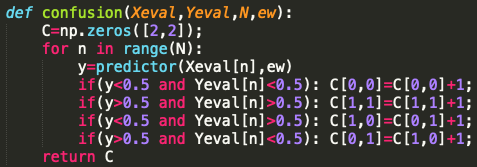
\includegraphics[width = 0.8\textwidth]{f_confusao.png}
  
  \caption {Função que calcula a matriz de confusão}
\end{figure}


\subsubsection{Accuracy}\hfill\newline
\hfill\newline

A implementação da accuracy passou por calcular usando a matriz de confusão quais as amostras corretamente classificadas e incorretamente classificadas pela ordem referida. e em seguida devolver o resultado da divisão do número de amostras bem classificadas pela totalidade das amostras classificadas (amostras bem classificadas + amostras mal classificadas).

\begin{figure}[H]

  \centering
  \captionsetup{justification=centering}

  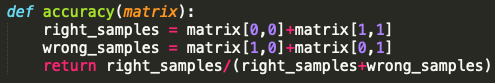
\includegraphics[width = 0.8\textwidth]{f_accuracy.png}
  
  \caption {Função que calcula a accuracy}
\end{figure}































\newpage
\section{Benchmarkting}

Nesta secção falar-se-á dos resultados obtidos e analisar-se-ão os mesmos. Vamos começar por apresentar a validação do classificador onde não se utilizaram janelas para remover o ruido e posteriormente serão apresentadas todas as janelas testadas com os respetivos filtros.\newline
É de sublinhar que cada uma das implementações testada foi corrida 9 vezes após a sua otimização, este processo é essencial uma vez que ao utilizarmos o método do gradiente estocástico inserimos um componente aleatório na convergência, ou seja é necessário realizar vários testes para garantir que este método não prejudica os resultados obtidos calibrando mal os pesos ou não permitindo a melhor calibração dos mesmos que se obteria por outros métodos mais precisos embora mais demorados.
Quanto á otimização levada a cabo em cada uma das versões do logistic classifier convêm referir algumas regras básicas que foram seguidas neste trabalho.
\begin{itemize}

	\item Devemos observar a variação do erro pós refinamento dos pesos para garantir que este não é errático o que indica que o learning rate é muito grande\cite{ref4}.
	\item É necessário verificar se o erro se torna estático durante algumas dezenas de epochs, este estaticismo revela que o número de epochs é demasiado elevado ou que o learning rate é demasiado baixo, no entanto caso este learning rate após dezenas de epochs em que a variação do erro tende a diminuir se tornar errático devemos truncar as epochs  até ao momento em que o erro se torna errático e repetir o refinamento dos pesos a partir dese ponto com um learning rate mais baixo\cite{ref4}.\hfill\newline
	\item Convêm saber que, por norma, o decréscimo do learning rate tende a situar-se algures entre 1/4 e 3/4 do valor anterior, verificando-se mais comummente o valor de 1/2, sendo este depois ajustado baseado nos resultados da progressão dos erros\cite{ref7}.
\end{itemize}


\subsection{Validação do Classificador}

Esta implementação trata-se do classificador genérico, este não faz uso nem de janelas deslizantes nem de filtros, em vez disso processa todas as imagens na sua totalidade. A progressão dos valores de erro e a tabela de confusão obtida após a otimização dos pesos do mesmo pode ser vista em baixo.

\begin{figure}[H]

  \centering
  \captionsetup{justification=centering}

  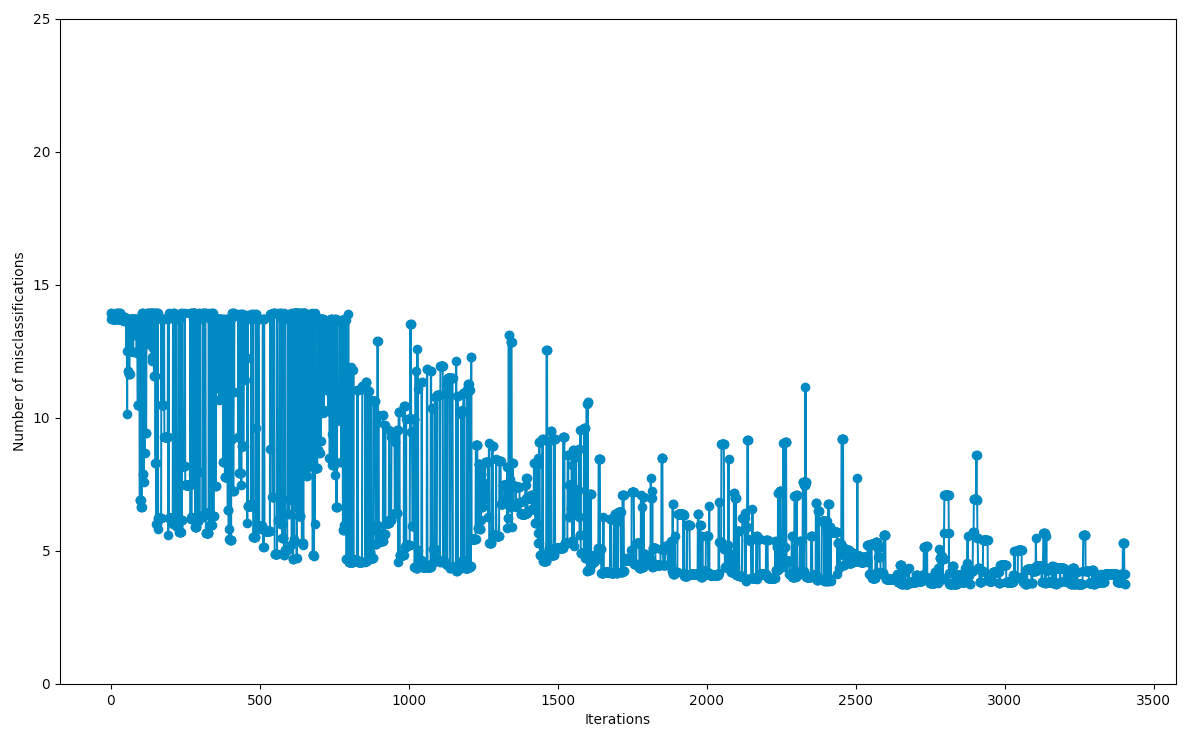
\includegraphics[width = 0.7\textwidth]{erros2_v1.png}
  
  \caption {Progressão dos erros da versão de validação}
\end{figure}

\begin{figure}[H]

  \centering
  \captionsetup{justification=centering}

  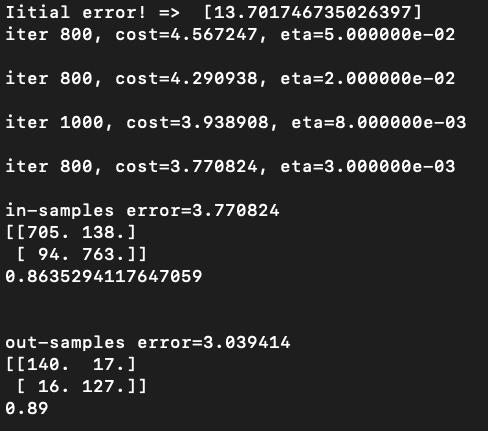
\includegraphics[width = 0.6\textwidth]{confusao2_v1.png}
  
  \caption {Tabelas de confusão da versão de validação}
\end{figure}


Como podemos ver na tabela de confusão do out-sample temos 300 imagens das quais 46 foram mal classificadas o que nos deixa com uma taxa de sucesso de 89\%. Através da representação dos erros no gráfico podemos verificar que a os erros tendem a estabilizar perto do valor 3,7 uma vez que a curva de otimização se comporta de tal forma que tende a estabilizar e a minimizar os ganhos em termos de taxa de sucesso face ao treino empregue após atingir este valor. Esta versão demora cerca de 23 minutos e 48 segundos a executar.\hfill\newline
Note-se também que existe underfitting dos dados de treino face aos dados de teste, indicando que caso o vetor de pesos seja usado para classificar um dataset de 3 e 8 maior os resultados não deverão desviar-se muito dos obtidos em cima embora possam piorar uma vez que o underfitting mostra que o modelo não se adaptou muito bem aos dados de treino.\newline
No presente momento podemos dizer que o dataset não é linearmente separável na sua totalidade uma vez que não conseguimos separar 11\% das imagens do out-sample.
 



\subsection{Análise dos Poolings Clássicos}

Nesta secção será abordada a utilização dos poolings denominados clássicos para avaliar os benefícios que estes fornecem á taxa de sucesso de previsão e aos tempos de execução do treino e teste do modelo. Estes serão apresentados na tabela abaixo pela mesma ordem em que foram implementados juntamente com os respetivos resultados\footnote{Para cada um dos poolings procedeu-se também a uma otimização dos parâmetros de learning rate e número de epochs.}. Note-se que, para cada combinação de janela e filtro de pooling, se realizaram 9 execuções do código e que o resultado apresentado é o melhor valor obtido dessas 9 execuções. Note-se também que as in-samples e out-samples serão referenciadas como $in$ e $out$ e que os seus valores estão em percentagem, e que os valores no campo time se encontram em minutos e segundos.

\begin{table}[h]
	\resizebox{\textwidth}{!}{ %
	\begin{tabular}{||c|c|c|c|c|c|c|c|c|c|c|c|c||}
	\hline
	\multirow{2}{*}{\backslashbox{Filtro}{Janela}}  & \multicolumn{3}{|c|}{2x2} & \multicolumn{3}{|c|}{2x3} & \multicolumn{3}{|c|}{3x2} & \multicolumn{3}{|c|}{3x3} \\ \cline{2-13}
	 &  \textbf{in}(\%) & \textbf{out}(\%) & \textbf{time}  & \textbf{in}(\%) & \textbf{out}(\%) & \textbf{time} &  \textbf{in}(\%) & \textbf{out}(\%) & \textbf{time} &  \textbf{in}(\%) & \textbf{out}(\%) & \textbf{time} \\ \hline


	Max           & 75,00 & 75,00 & 17:00 & 67,40 & 69,00 & 11:38 & 66,94 & 69,00 & 8:48 & 88,00 & 88,67 & 6:32 \\ \hline
	Min           & 86,00 & 89,30 & 16:09 & 88,18 & 90,00 & 9:11 & 87,71 & 90,00 & 11:40 & 89,88 & 90,33 & 6:34 \\ \hline
	Average       & 85,70 & 85,67 & 17:46 & 84,18 & 86,67 & 9:52 & 78,65 & 83,33 & 12:52 & 83,06 & 82,33 & 3:04 \\ \hline
	Max Centered  & 88,60 & 88,30 & 21:02 & 88,06 & 90,00 & 13:58 & 88,00 & 90,00 & 8:32 & 86,29 & 89,00 & 6:51 \\ \hline

	\end{tabular}%
	}
\end{table}


\begin{table}[h]
	\centering
	\resizebox{0.6\textwidth}{!}{ %
	\begin{tabular}{||c||c|c|c|c|c|c|c|c|c|c|c|c||}
	\hline
	\multirow{2}{*}{Validação do Classificador}    & in-sample(\%) & out-sample(\%) & time  \\\cline{2-4}
	& 86,35 & 89,00 & 23:48 \\\hline

	\end{tabular}%
	}
\end{table}


Nesta tabela temos vários resultados que se mostram melhores que os obtidos aquando da validação do classificador, sendo que esses resultados são fruto da conjugação dos filtros "Min" e "Max Centered" com as várias janelas utilizadas. Por outro lado o filtro "Max" teve maus resultados conjugado com todas as janelas exceto a 3x3. \newline
No caso do filtro Min podemos observar que á medida que aumentamos as dimensões da janela os resultados tendem a melhorar e o underfitting do modelo tende a diminuir, sendo o seu menor valor 0.45\% no caso da janela 3x3. O modelo resultante da conjugação do fitro Min com a janela 3x3 e stride 2 nas dimensões x e y foi aquele que produziu o melhor resultado uma vez que apresenta juntamente com a melhor taxa de sucesso nas previsões, a menor taxa de underfitting e o melhor tempo demorando apenas 6 minutos e 34 segundos a executar.\newline
É também importante realçar que comparando os resultados obtidos das conjugações dos diferentes filtros empregues com as janelas 2x3 e 3x2 se verifica que a janela 2x3 é em geral melhor para prever os dados por possuir menor underfitting, isto é as imagens do dataset são melhor classificadas caso se use uma janela que possua dimensões em $y$ maiores do que em $x$.



\subsection{Análise dos Poolings Exóticos}

Nesta secção será analisada a utilização dos poolings exóticos implementados e explicados na secção anterior. Mais uma vez executaram-se 9 vezes cada combinação de janela e filtro e apenas o melhor resultado de cada combinação é apresentado. Adicionalmente sublinha-se que as in-samples e out-samples encontram-se na tabela referenciadas como $in$ e $out$ e os seus valores encontram-se em percentagem. Uma vez que os nomes dos filtros exóticos são extensos utilizar-se-ão as iniciais de cada um e estes serão apresentados na tabela pela ordem de apresentação dos mesmos na subsecção~\ref{subsec:poolingExotico}. 


\begin{table}[h]
	\resizebox{\textwidth}{!}{ %
	\begin{tabular}{||c|c|c|c|c|c|c|c|c|c|c|c|c||}
	\hline
	\multirow{2}{*}{\backslashbox{Filtro}{Janela}}  & \multicolumn{3}{|c|}{2x2} & \multicolumn{3}{|c|}{2x3} & \multicolumn{3}{|c|}{3x2} & \multicolumn{3}{|c|}{3x3} \\ \cline{2-13}
	 &  \textbf{in}(\%) & \textbf{out}(\%) & \textbf{time}  & \textbf{in}(\%) & \textbf{out}(\%) & \textbf{time} &  \textbf{in}(\%) & \textbf{out}(\%) & \textbf{time} &  \textbf{in}(\%) & \textbf{out}(\%) & \textbf{time} \\ \hline

 DVAP & 83,65 & 87,00 & 13:03 & 84,18 & 87,00 & 6:24 & 84,18 & 87,00 & 6:35 & 81,06 & 82,00 & 5:33 \\ \hline
DVMCP & 89,24 & 87,67 & 15:43 & 84,29 & 86,67 & 6:40 & 88,76 & 90,00 & 6:57 & 86,59 & 90,33 & 6:54 \\ \hline
 DVMP & 86,35 & 90,33 & 20:33 & 88,67 & 83,41 & 8:37 & 85,82 & 89,33 & 8:58 & 87,53 & 89,00 & 4:26 \\ \hline
DVMAP & 86,12 & 89,67 & 21:33 & 86,12 & 87,67 & 10:07 & 85,76 & 88,33 & 8:30 & 83,88 & 85,00 & 4:42 \\ \hline

	\end{tabular}%
	}
\end{table}

\begin{table}[h]
	\centering
	\resizebox{0.6\textwidth}{!}{ %
	\begin{tabular}{||c||c|c|c|c|c|c|c|c|c|c|c|c||}
	\hline
	\multirow{2}{*}{Validação do Classificador}    & in-sample(\%) & out-sample(\%) & time  \\\cline{2-4}
	& 86,35 & 89,00 & 23:48 \\\hline

	\end{tabular}%
	}
\end{table}


No geral os resultados obtidos com a aplicação dos poolings exóticos são inferiores aos obtidos com poolings clássicos. No entanto, existem 2 resultados que superam os anteriormente vistos, nomeadamente a conjugação do filtro Diagonal and Vertical Max Pooling com a janela 2x2 e do filtro Diagonal and Vertical Max Centered Pooling com a janela 3x3. Embora ambos tenham um resultado de out-sample igual, o segundo pooling referido oferece 2 vantagens face ao primeiro. Além de possuir um underfitting ligeiramente inferior é pelo menos três vezes mais rápido a executar fazendo deste a escolha obvia como o melhor modelo dos dois.\newline
\hfill\newline
Comparando todos os resultados obtidos durante os testes podemos concluir que o melhor modelo se trata daquele resultante da aplicação do filtro "Min" á janela 3x3 por se tratar do mais rápido com menor underfitting e melhor valor preditivo. Adicionalmente podemos concluir que cerca de 9-10\% desta base de dados não é linearmente separável, totalizando cerca de 27-30 imagens do dataset de treino as quais o nosso melhor modelo não consegue separar. 

Adicionalmente procurou-se saber qual a janela minima a utilizar para se verificar uma perda total de informação útil para além de ruido. Verificou-se que a perda de informação útil se começa a dar a partir da janela de dimensões 6x5 com strides 5 em x e 4 em y. \newline
O cenário onde se verificou a perda total de informação útil deu-se quando se utilizou uma janela de tamanho 10x9 com strides 9 em x e 8 em y, resultando em imagens de 9 pixeis quase impossiveis de se distinguirem como se pode verificar na matriz de confusão obtida.

\begin{figure}[H]
	
\captionsetup{justification=centering}
  \begin{subfigure}{.5\textwidth}
  \centering
  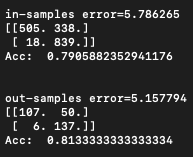
\includegraphics[width = 0.6\textwidth]{first_result.png}
  \caption {Tabelas de confusão da janela 6x5}
  \end{subfigure}
  \begin{subfigure}{.5\textwidth}
  \centering
  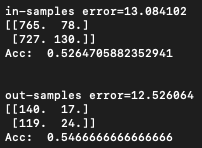
\includegraphics[width = 0.67\textwidth]{worst_result.png}
  \caption {Tabelas de confusão da janela 10x9}
  \end{subfigure}
\end{figure}



















\newpage

%
% ---- Bibliography ----
%
% BibTeX users should specify bibliography style 'splncs04'.
% References will then be sorted and formatted in the correct style.
%
% \bibliographystyle{splncs04}
% \bibliography{mybibliography}
%
\begin{thebibliography}{8}

%\bibitem{ref_intro1}
%https://www.itu.int/en/ITU-D/Statistics/Pages/stat/default.aspx
\bibitem{ref1} Ian Goodfellow, Yoshua Bengio and Aaron Courville. \href{http://www.deeplearningbook.org/contents/TOC.html}{\textit{Deep Learning}}. MIT Press, 2016.
\bibitem{ref2} Kevin P. Murphy. \textit{Machine Learning: A Probabilistic Perspective}. MIT Press, 2012.
\bibitem{ref3} Trevor Hastie, Robert Tibshirani and Jerome Friedman. \textit{The Elements of Statistical Learning Data Mining, Inference, and Prediction}. Springer, Janeiro 13 de 2017.
\bibitem{ref4} John D. Keller, Brian Mac Namee and Aoife D'Arcy. \textit{Fundamentals of Machine Learning For Predictive Data Analytics}. MIT Press, 2015.
\bibitem{ref5} Mehryar Mohri, Afshin Rostamizadeh and Ameet Talwalkar. \textit{Foundations of Machine Learning}. MIT Press, 2018.
\bibitem{ref6} Josh Hugh Learning. \textit{Python Machine Learning}. JHL.
\bibitem{ref7} Charu C. Aggarwal. \textit{Linear Algebra and Optimization for Machine Learning}. Springer, 2020.
\bibitem{ref8} Ivan Vasilev, Daniel Slater, Gianmario Spacagna, Peter Roelants and Valentino Zocca. \textit{Python Deep Learning}. Packt, 2019.
\bibitem{ref9} Nathalie Japkowicz. \textit{Evaluating Learning Algorithms: A Classification Perspective}. cambridge university press, 2011.
\end{thebibliography}
%\input{anexo.tex}

\end{document}